% ============================================================================
\section{Hardware Components}
\label{sec:hardware}
% ============================================================================

\subsection{Bill of materials (Wokwi parts)}
The circuit is \file{firmware/diagram.json}: 20 electronic parts plus 14 text labels.

{\small
\begin{longtable}{@{}p{0.25\linewidth}cp{0.62\linewidth}@{}}
\toprule
Part (Wokwi type) & Qty & Purpose \\
\midrule
\endhead
ESP32-S3-DevKitC-1 & 1 & Microcontroller: dual-core Xtensa LX7 at 160\,MHz, runs all terminals. \\
\multicolumn{3}{@{}l}{\emph{Entrance terminal}} \\
MFRC522 RFID reader (\code{board-mfrc522}) & 2 & Entry reader and exit reader, 13.56\,MHz
  ISO 14443\,A cards, SPI. Wokwi provides the cards (\cref{sec:rfid-cards}). \\
Servo motor & 2 & Door locks: entry door and exit door (0\textdegree{} closed,
  90\textdegree{} open). \\
LCD 20$\times$4 (I2C, 0x27) & 1 & Status display and messages (\cref{sec:op-ui}). \\
Buzzer & 1 & Audible feedback: granted, denied, information, alarm. \\
LED (green) + 220\,$\Omega$ resistor & 1 & ``Access granted'' indicator, on for 2\,s. \\
Push button (key \code{e}) & 1 & Break-glass emergency: opens both doors. \\
DS1307 RTC (I2C, 0x68) & 1 & Real-time clock, so the schedule works without a network. \\
microSD card (SPI) & 1 & Event log storage (\req{2.4}). \\
\multicolumn{3}{@{}l}{\emph{Each lecture room (2 sets)}} \\
PIR motion sensor & 1 & Occupancy detection. \\
Photoresistor (LDR) module & 1 & Ambient light in lux, read on the analog output (ADC1). \\
LED (white) + resistor & 1 & The room's lamp, dimmed by PWM. \\
\bottomrule
\end{longtable}
}

\paragraph{RFID readers and cards.}
\label{sec:rfid-cards}
The entrance has two MFRC522 readers: the \textbf{entry reader} (people coming in) and the
\textbf{exit reader} (people going out), each beside its own door. In Wokwi, clicking a reader
opens its control panel: choose a card and press \textbf{Tap} (the card is held to the reader
for 0.5\,s) or \textbf{Hold}. The preset cards are registered as the demo users:

\begin{center}
\small
\begin{tabular}{@{}llll@{}}
\toprule
Wokwi card & UID & Registered as & Role \\
\midrule
Blue   & \code{01:02:03:04} & Alice & STUDENT \\
Green  & \code{11:22:33:44} & Bob   & STAFF \\
Yellow & \code{55:66:77:88} & Carol & SECURITY \\
Red    & \code{AA:BB:CC:DD} & Admin & ADMIN (PIN \code{1234}) \\
Key fob & \code{C0:FF:EE:99} & -- (unregistered) & -- \\
NFC tag & \code{04:11:22:33:44:55:66} & -- (unregistered) & -- \\
\bottomrule
\end{tabular}
\end{center}
The rest of the system only ever sees ``card \emph{UID} scanned at side \emph{IN/OUT}''
(\file{components/nodes/include/rfid.h}), so any UID, including unregistered ones, can also be
scanned from the CLI with \code{tap <UID> in|out}.

\subsection{Pin map}
\file{components/common/include/board_pins.h} is the single source of truth. Pins follow the
board's physical header order, which keeps the wiring tidy (\cref{sec:wiring}).

{\small
\begin{longtable}{@{}llll@{}}
\toprule
Header & Function & GPIO & Notes \\
\midrule
\endhead
left  & Room 1: LDR / PIR / lamp & 4 / 5 / 6 & LDR on ADC1\_CH3 \\
left  & Room 2: LDR / PIR / lamp & 7 / 15 / 16 & LDR on ADC1\_CH6 \\
left  & SD card MISO / SCK / MOSI / CS & 10 / 11 / 12 / 13 & SPI2 (SD card only) \\
left  & Buzzer & 14 & LEDC PWM \\
right & Entry reader SDA (chip select) & 1 & SPI3 \\
right & RFID SCK / MOSI / MISO & 2 / 42 / 41 & SPI3, shared by both readers \\
right & RFID RST & 40 & both readers, active low \\
right & Exit reader SDA (chip select) & 39 & SPI3 \\
right & I2C SDA / SCL (LCD, RTC) & 36 / 35 & one shared bus \\
right & Entry / exit door servo & 48 / 47 & LEDC 50\,Hz \\
right & Break-glass button & 21 & pull-up, interrupt \\
right & ``Access granted'' LED & 20 & \\
\bottomrule
\end{longtable}
}

\paragraph{Peripheral sharing.} The SD card has SPI bus~2 to itself; the two readers share
SPI bus~3 and are told apart by their chip-select pins, so a card read never waits for an SD write.
The LCD and RTC share one I2C bus (different addresses). The ESP32
LED controller (LEDC) provides all PWM: timer~0 at 50\,Hz for both servos, timer~1 at 5\,kHz for
the two lamps, and timer~2 for the buzzer, whose frequency changes per tone. The two light sensors
share ADC unit~1, protected by a mutex (\cref{sec:sync}).

\subsection{Wiring}
\label{sec:wiring}
\Cref{fig:wokwi} shows the complete circuit in Wokwi; \cref{fig:wokwi-parts} shows the entrance,
a reader's control panel and a lecture room.

\screenshot{wokwi}{The complete circuit running in the Wokwi simulator.}
  {Whole Wokwi canvas while the simulation runs (zoom out until every part is visible).}

\begin{figure}[H]
\centering
\begin{minipage}[c]{0.36\linewidth}
  \centering
  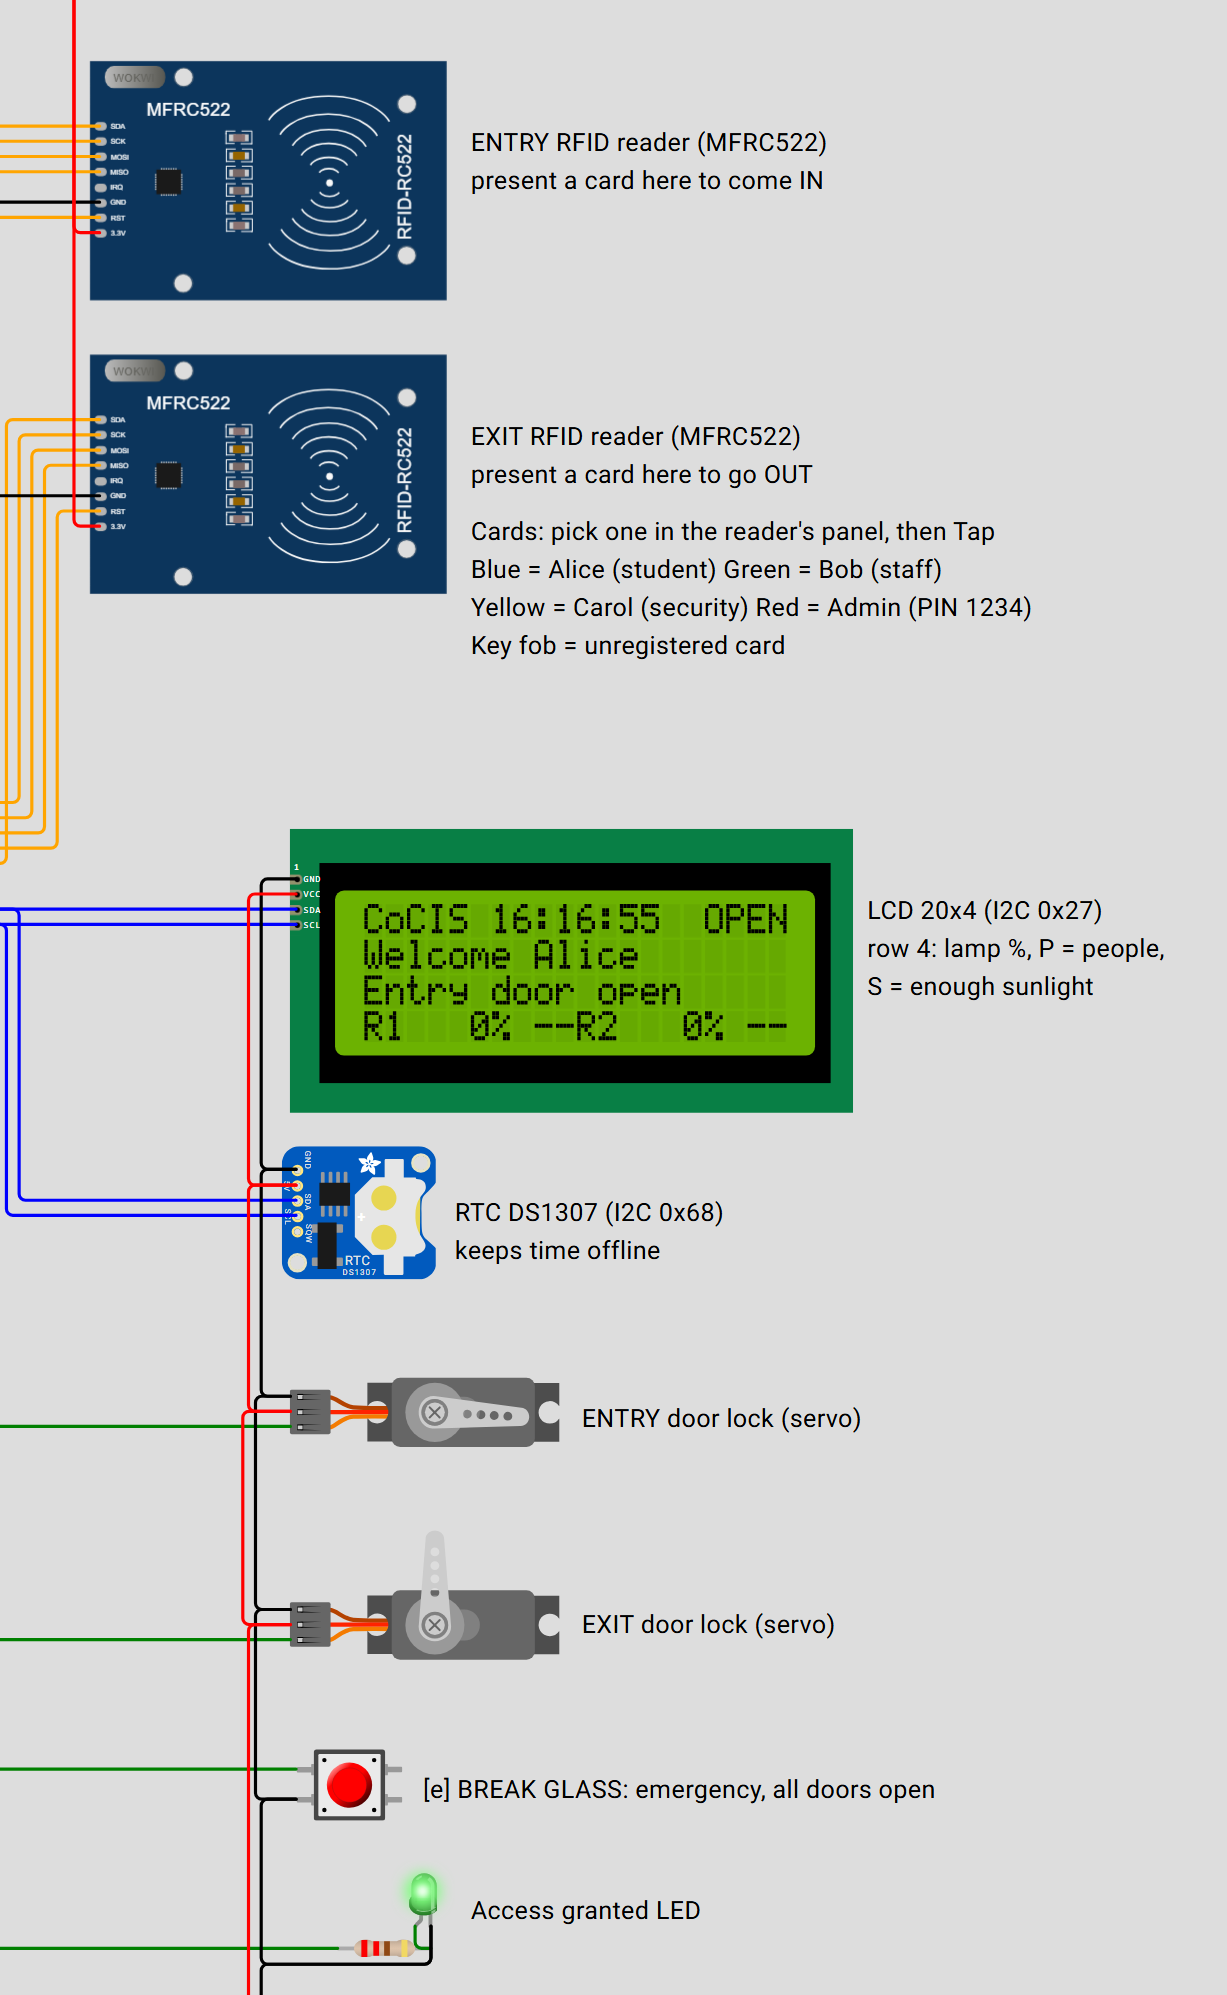
\includegraphics[width=\linewidth]{wokwi-entrance.png}\\[2pt]
  {\small (a) Entrance terminal}
\end{minipage}\hfill
\begin{minipage}[c]{0.6\linewidth}
  \centering
  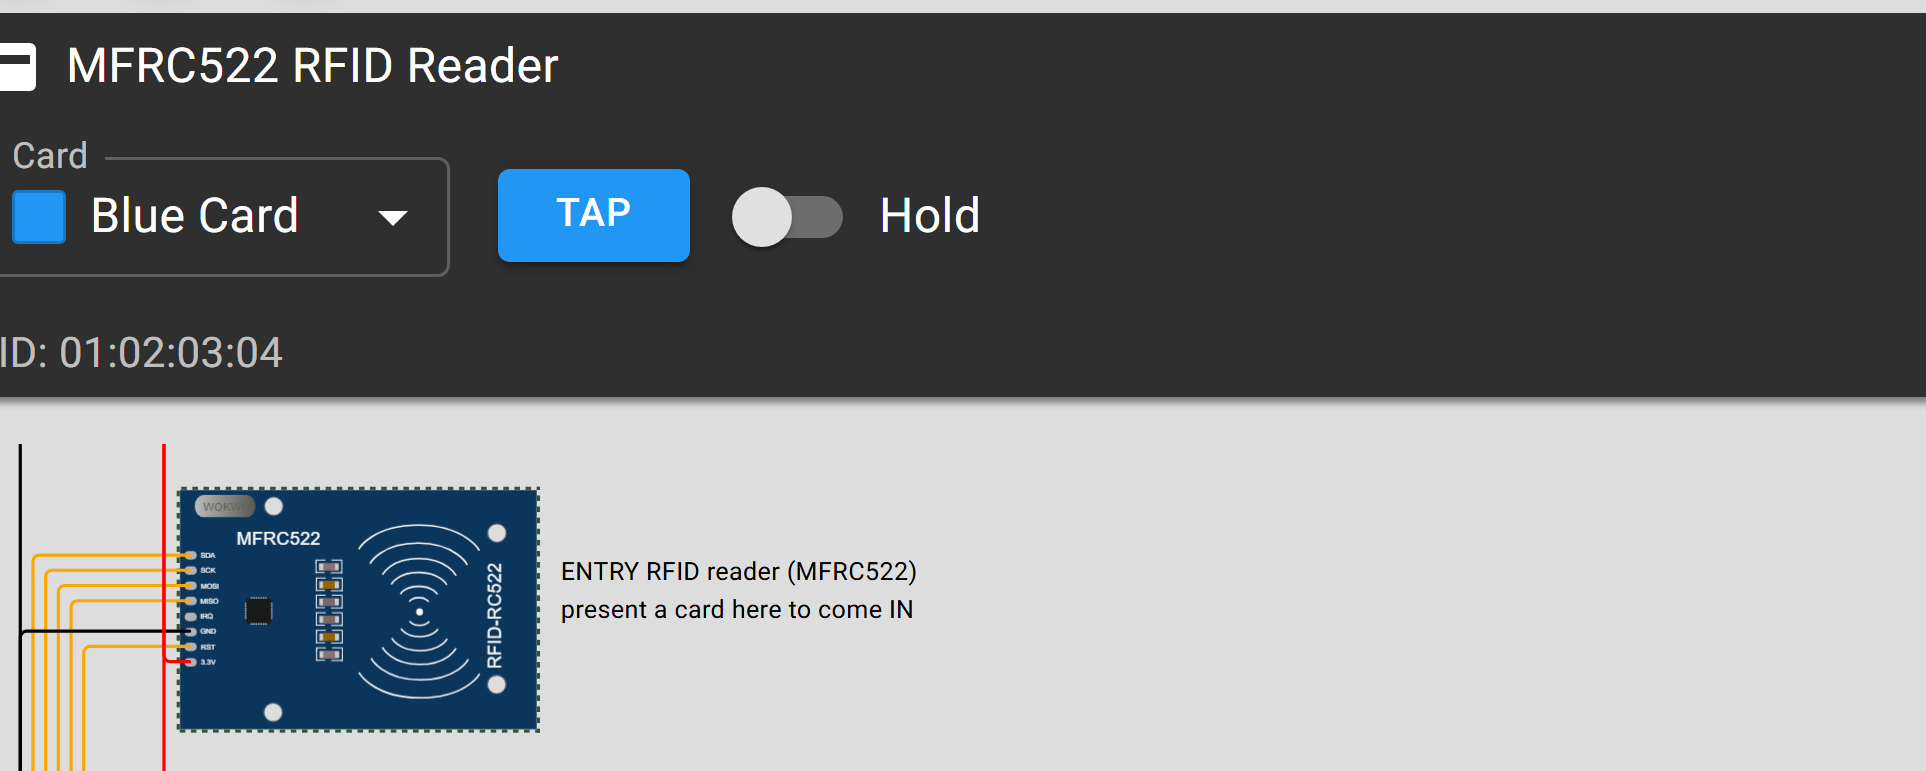
\includegraphics[width=\linewidth]{wokwi-reader.png}\\[2pt]
  {\small (b) A reader's control panel: pick a card, then Tap or Hold}\\[10pt]
  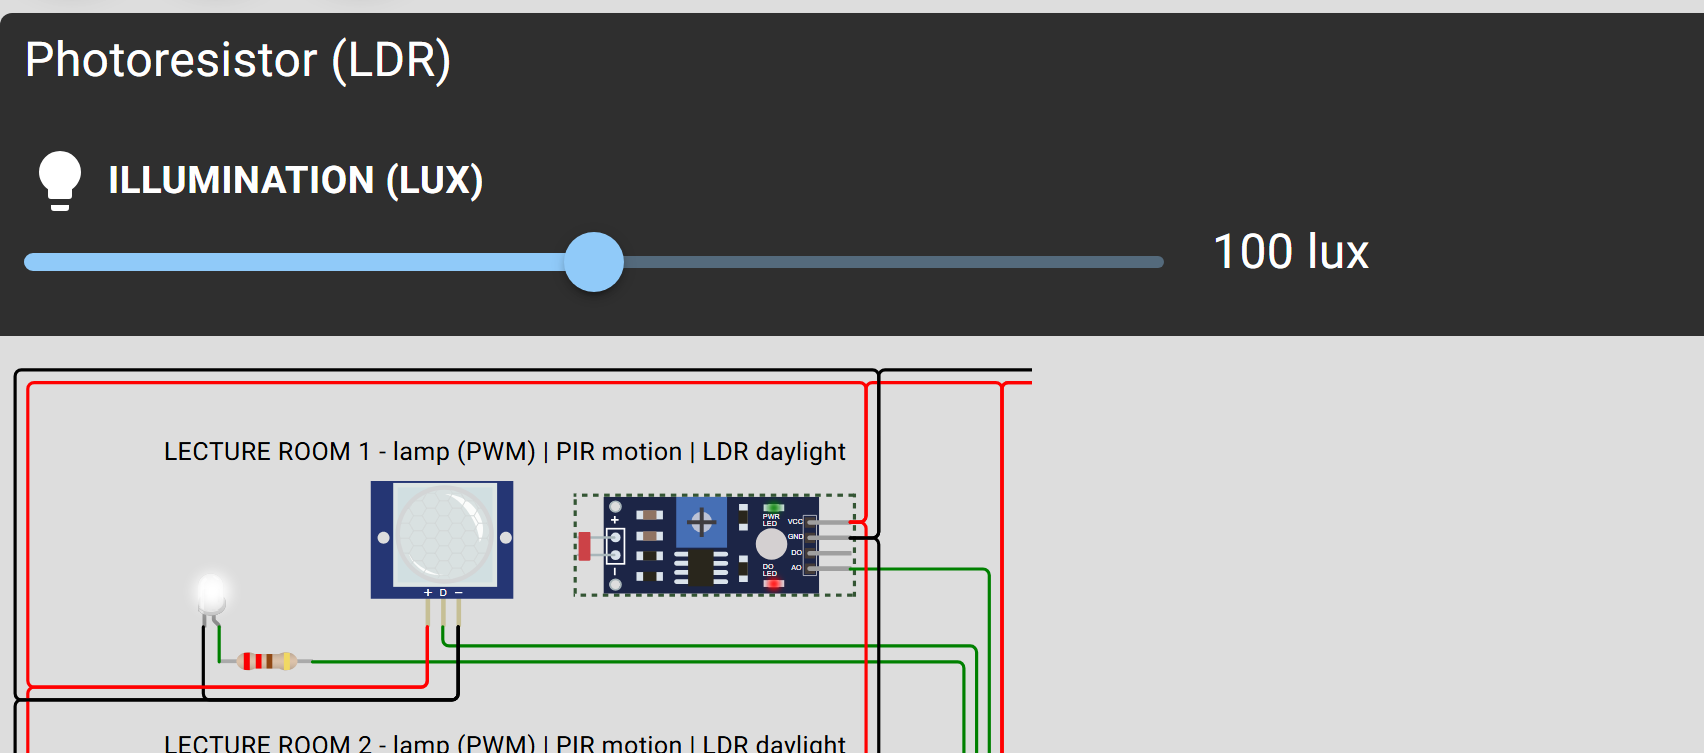
\includegraphics[width=0.9\linewidth]{wokwi-room.png}\\[2pt]
  {\small (c) Lecture room 1: lamp on, light-sensor panel open}
\end{minipage}
\caption{Parts of the circuit in Wokwi. (a) The entrance: entry and exit RFID readers, LCD, RTC,
door servos, break-glass button and granted LED. (b) Clicking a reader opens its panel.
(c) A lecture room: PIR sensor, light sensor and lamp; clicking a sensor opens its controls.}
\label{fig:wokwi-parts}
\end{figure}
